\section{Foundations and Analytical Framework}
\label{sec:framework}
\begin{figure}[t]
\centering
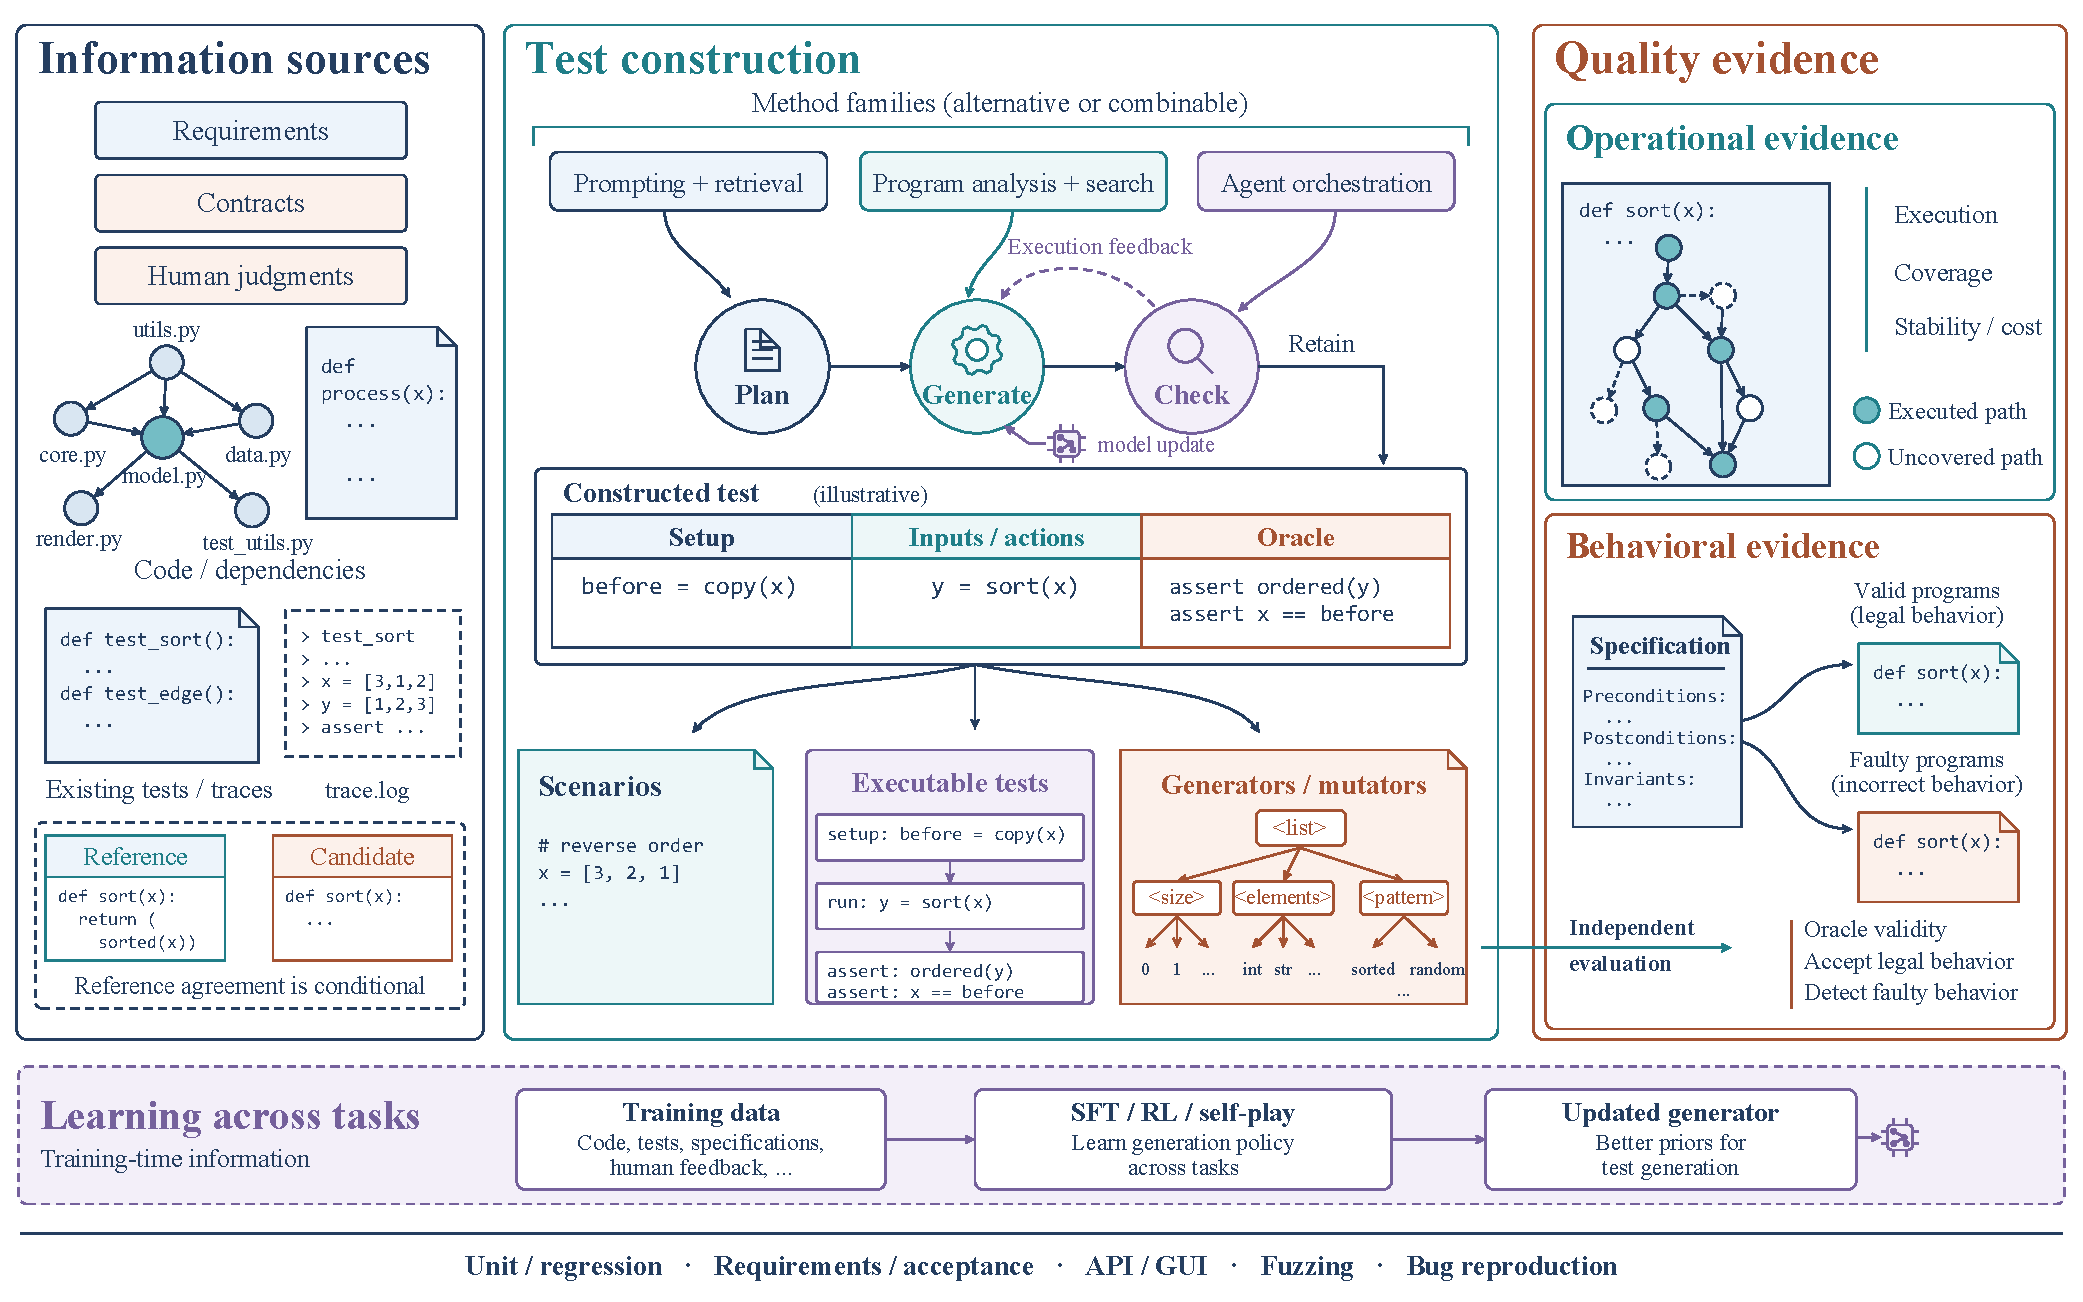
\includegraphics[width=\linewidth]{figures/construction-overview-illustrated.pdf}
\caption{A synthesis of LLM-based test generation. Information sources support planning, generation, and checking; alternative or combined mechanisms construct scenarios, executable tests, and generators. The sorting sketch illustrates setup, action, and a partial oracle. Dashed feedback revises the current artifact; matching violet model icons connect the cross-task learning output to generation. Operational and behavioral evidence address different quality properties. Independent evaluation supplies held-out evidence without feeding its results back into generation.}
\Description{Three separate requirement, contract, and human-judgment cards appear above code dependencies, existing tests and traces, and reference and candidate programs. Planning, generation, and checking construct an illustrative sorting test with setup, action, and oracle. Three output branches show scenarios, executable tests, and generators. A separate training lane supplies an updated model, represented by matching model-chip icons. Operational path evidence and independent behavioral evaluation occupy the right-hand panel.}
\label{fig:overview}
\end{figure}
\subsection{What Is Generated?}
An executable test combines a setup, an input or action sequence, and an oracle that judges the resulting behavior. Its setup can include fixtures, mocks, dependencies, credentials, database state, and cleanup. Its input may be a function argument, an HTTP request, a GUI action, or an entire generated program. Its oracle may check an exact output, an exception, a relation across executions, or a safety property. A test suite additionally determines which tests coexist, how state is isolated, and when execution ends.

Many generation methods produce an intermediate artifact. A natural-language scenario still requires operationalization. A grammar defines a family of admissible inputs but does not necessarily determine their expected outputs. A fuzzing driver connects generated data to a target API while relying on a separate failure detector. We therefore distinguish \emph{test design}, \emph{test input}, \emph{test oracle}, \emph{executable test}, and \emph{test-generation infrastructure}. This distinction preserves the contributions of input-only and infrastructure methods without attributing complete test synthesis to them.

\subsection{Testing Objectives Determine Oracle Roles}
Functional conformance asks whether behavior satisfies an external requirement. Regression testing asks whether a change violates behavior that should be preserved. Bug reproduction asks whether a reported failure can be exercised and distinguished from its repair. Fuzzing often searches for crashes, sanitizer violations, or disagreement among implementations. Tests used in code generation may instead rank candidate solutions or provide debugging feedback. These objectives can share execution machinery while requiring different oracle evidence.

Consider a requirement that a function return a sorted permutation of its input without modifying the input. A test may assert the sorted result yet omit the mutation constraint. It can execute successfully and reach every line while leaving part of the requirement unchecked. A test copied from an implementation that sorts in place can even preserve the very violation that a conformance test should reveal. Conversely, a test that expects one particular ordering among equal-key objects may reject a legal implementation if stability was never required. This illustrative example motivates evaluating both detection of invalid behavior and acceptance of permitted behavior.

\subsection{Information Access and Correctness Evidence}
We distinguish three stages of information access: training, generation, and final evaluation. At each stage, relevant sources include requirements, focal code, repository context, existing tests, reference implementations, candidate implementations, execution traces, and human decisions. Access is a property of an experimental variant rather than an entire paper. For instance, inference can use a description and signature even when training rewards require a reference program, as in PyTester~\cite{T01}. Describing that configuration simply as ``code-free'' would erase a material dependency.

An information source can play more than one role. Source code helps resolve imports and construct objects; the same code can also supply expected outputs. A static dependency graph can identify callable APIs without validating their semantics. Execution of a trusted reference provides a concrete output under the reference assumption. Execution of the candidate under test provides an observation about that candidate. These roles should be recorded separately because context relevance and oracle independence answer different questions.



Figure~\ref{fig:overview} connects the four dimensions of our analytical framework: objectives and artifacts, information access, generation mechanisms, and quality evidence. The dimensions are intentionally orthogonal. ``Agent-based'' describes how decisions are coordinated; ``requirements-based'' describes an information source; ``unit testing'' describes a testing level. Treating these labels as competing branches of one taxonomy would place overlapping studies in arbitrary categories. We instead use testing settings to organize the landscape and mechanisms to explain recurring design choices.
